\section{ARIFI's project description}
ARIFI is an ongoing project whose main goal is to combine GNSS services with Artificial intelligence into a web application. This application will provide agricultors not only with useful data, but also with instructions on what actions to take so as to manage more efficiently their farms and improve their harvest profits.\\
%
%
The project started after a several discussions with farmers from different countries around the world. The intention of this conversations via phone calls or e-mail, was to get a deeper insight on the current agriculture situation. We tried to analyse common difficulties among farmers, despite being far apart from one another, making special emphasis in those that we thought we contribute to, as a team with solid knowledge in GNSS and AI.\\
%
%
In conclusion, we obtained valuable feedback from farmers that helped the team to better shape the project and define more clearly which difficulties we wanted to adress with ARIFI. The later have been itemized and briefly described next, so as to give a more schematic look of what we concluded.
% REVISAAAAAAAAAAAAAAR JOAN
%::::::::::::::::::
%::::::::::::::::::
%::::::::::::::::::
\begin{itemize}
    \item \textbf{Interpretation of weather forecasts:} It is well known that weather forecasts are of extreme importance for agriculture. It helps farmers to prevent their harvest to be damaged and also to adapt system such as irrigation. In this case, we found that the forecasts most farmers obtained were not detailed enough in many cases, and more importantly, most of them were only useful for well experienced agricultors which knew to interpret this information and what actions to take in result. This is a problem that ARIFI wants to solve by gathering all the necessary data, not only to make weather forecasts, but also to combine it with data from other sources so as to provide users with instructions on how to act even if they are not well experienced farmers. This can be specially useful in the agriculture sector from developing countries that lack from technical advise from specialized companies. 
    \item \textbf{knowledge of field's characteristics:} Although all farmers know their fields to some extend, not many have detailed knowledge about aspects, e.g. soil height irregularities, chemical characteristics etc, which are relevant for many farming activities. This characteristics are currently not easy to determine and in some cases it implies expensive measurings processes that might take long. In this aspect ARIFI wants to provide with useful information by processing copernicu's images.
    \item \textbf{Adaptation to climate change:}
\end{itemize}

\subsection{Project overview}
%
\begin{figure}[b!]
    \centering
    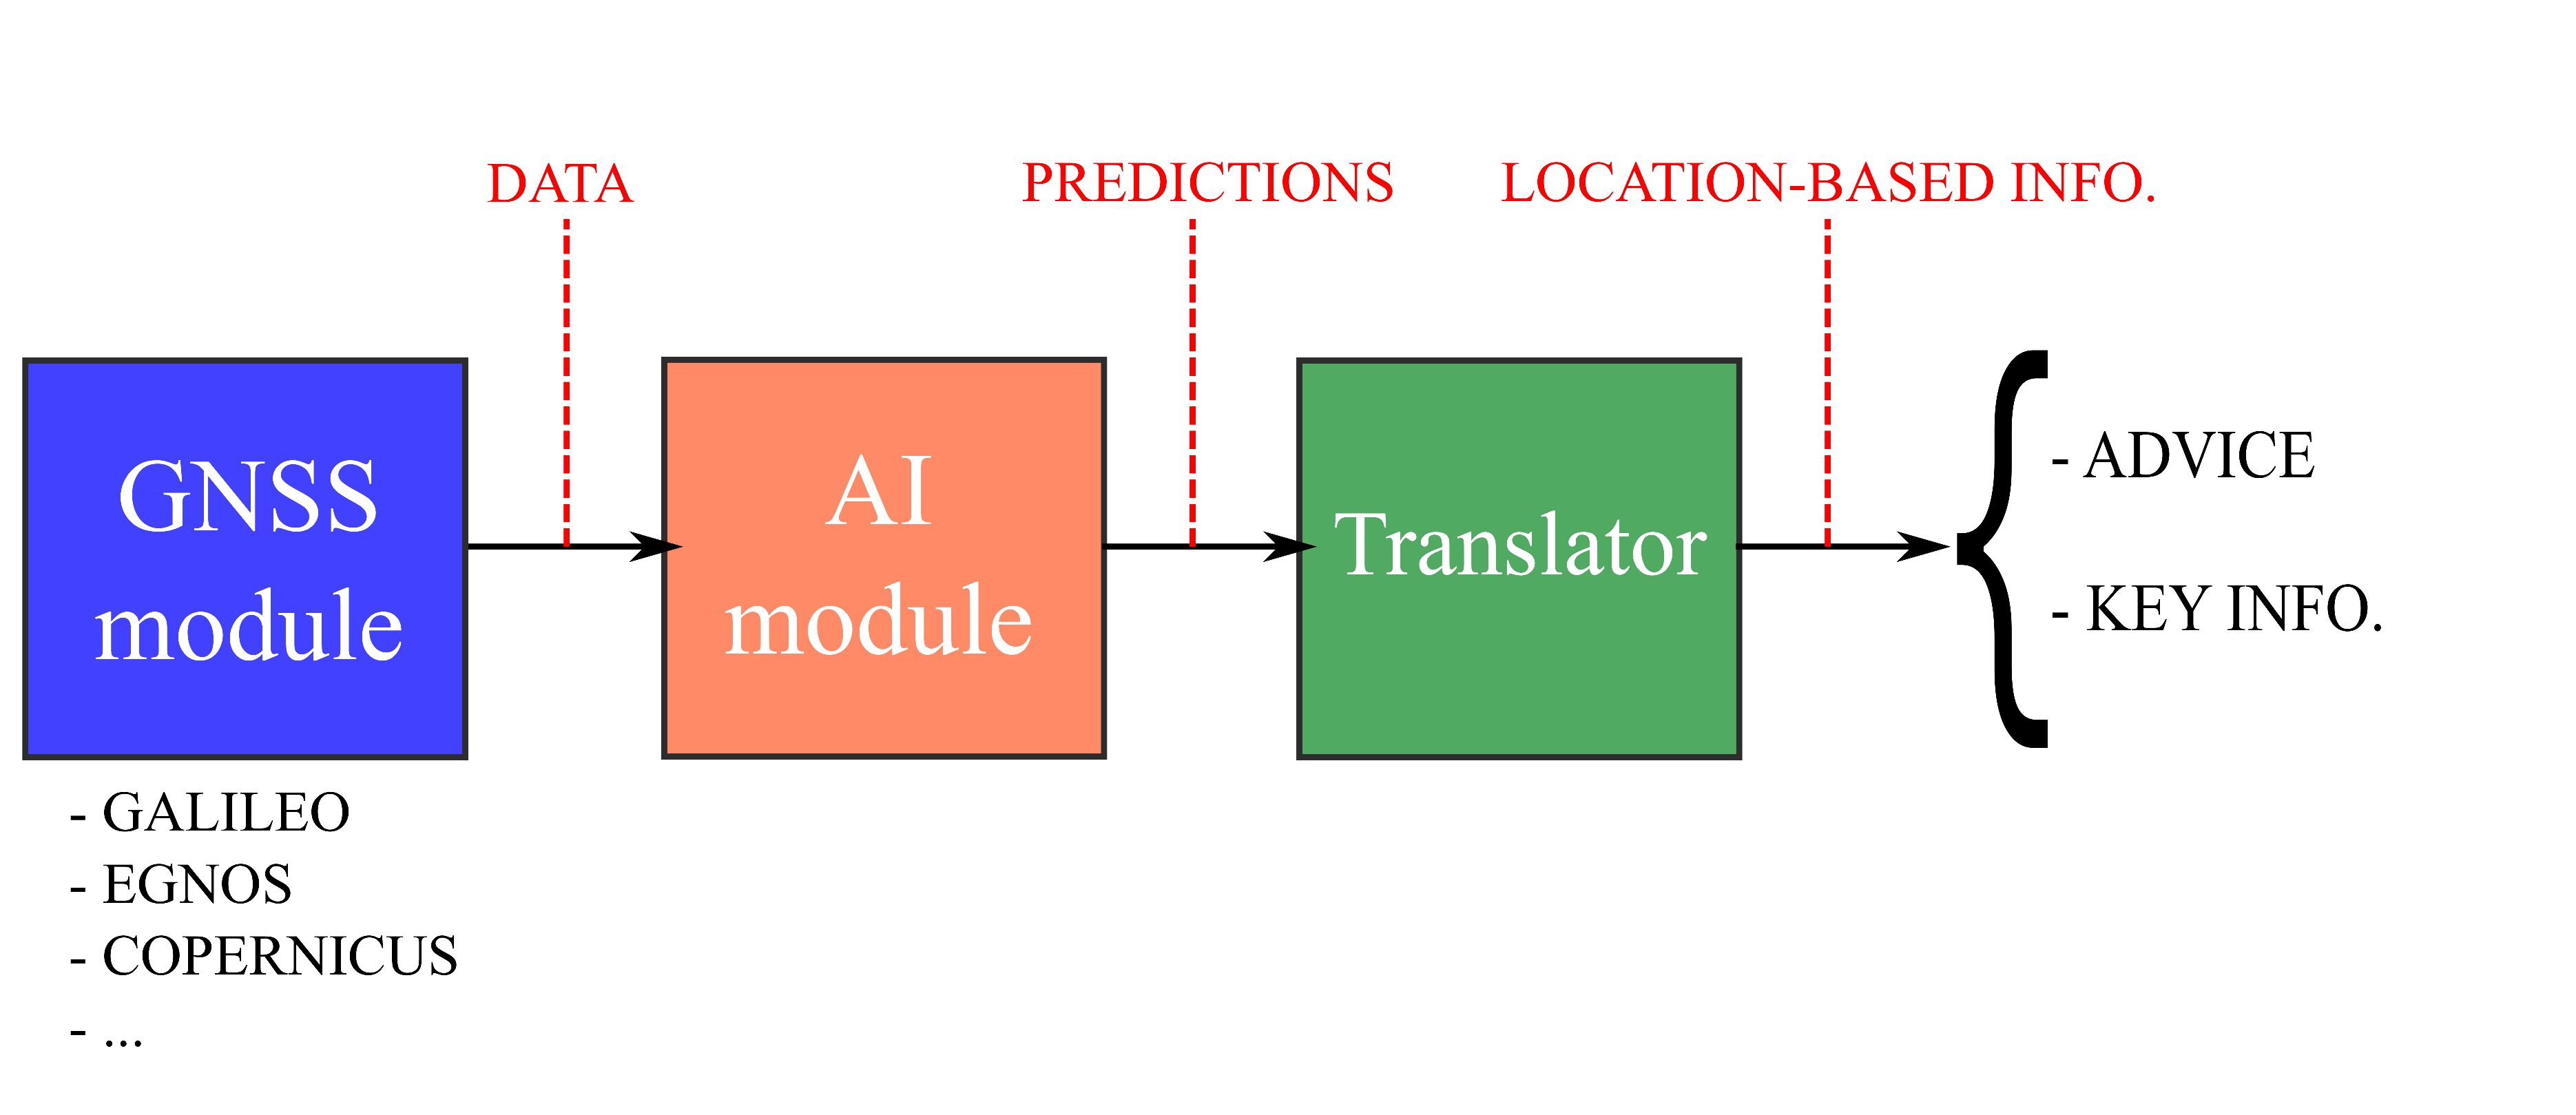
\includegraphics[scale= 0.26]{images/dibujo1.eps}
    \caption{ARIFI's general schematic}
    \label{fig:sch1}
\end{figure}
%
The principal idea is that GNSS together with other sources act as data providers to ARIFI's AI module, which will collect and integrate this information to its algorithm. Next, the AI module will output a prediction of key parameters, that will be later interpreted and made understandable for agricultors. This part is where ARIFI specially stands out from other services, as it will make special emphasis in translating AI predictions into instructions for farmers, so that their harvest follows a more efficient agricultural plan. In figure \ref{fig:sch1}, it is displayed an schematic idea of ARIFI's general concept.\\\\
%
\begin{figure}[t!]
    \centering
    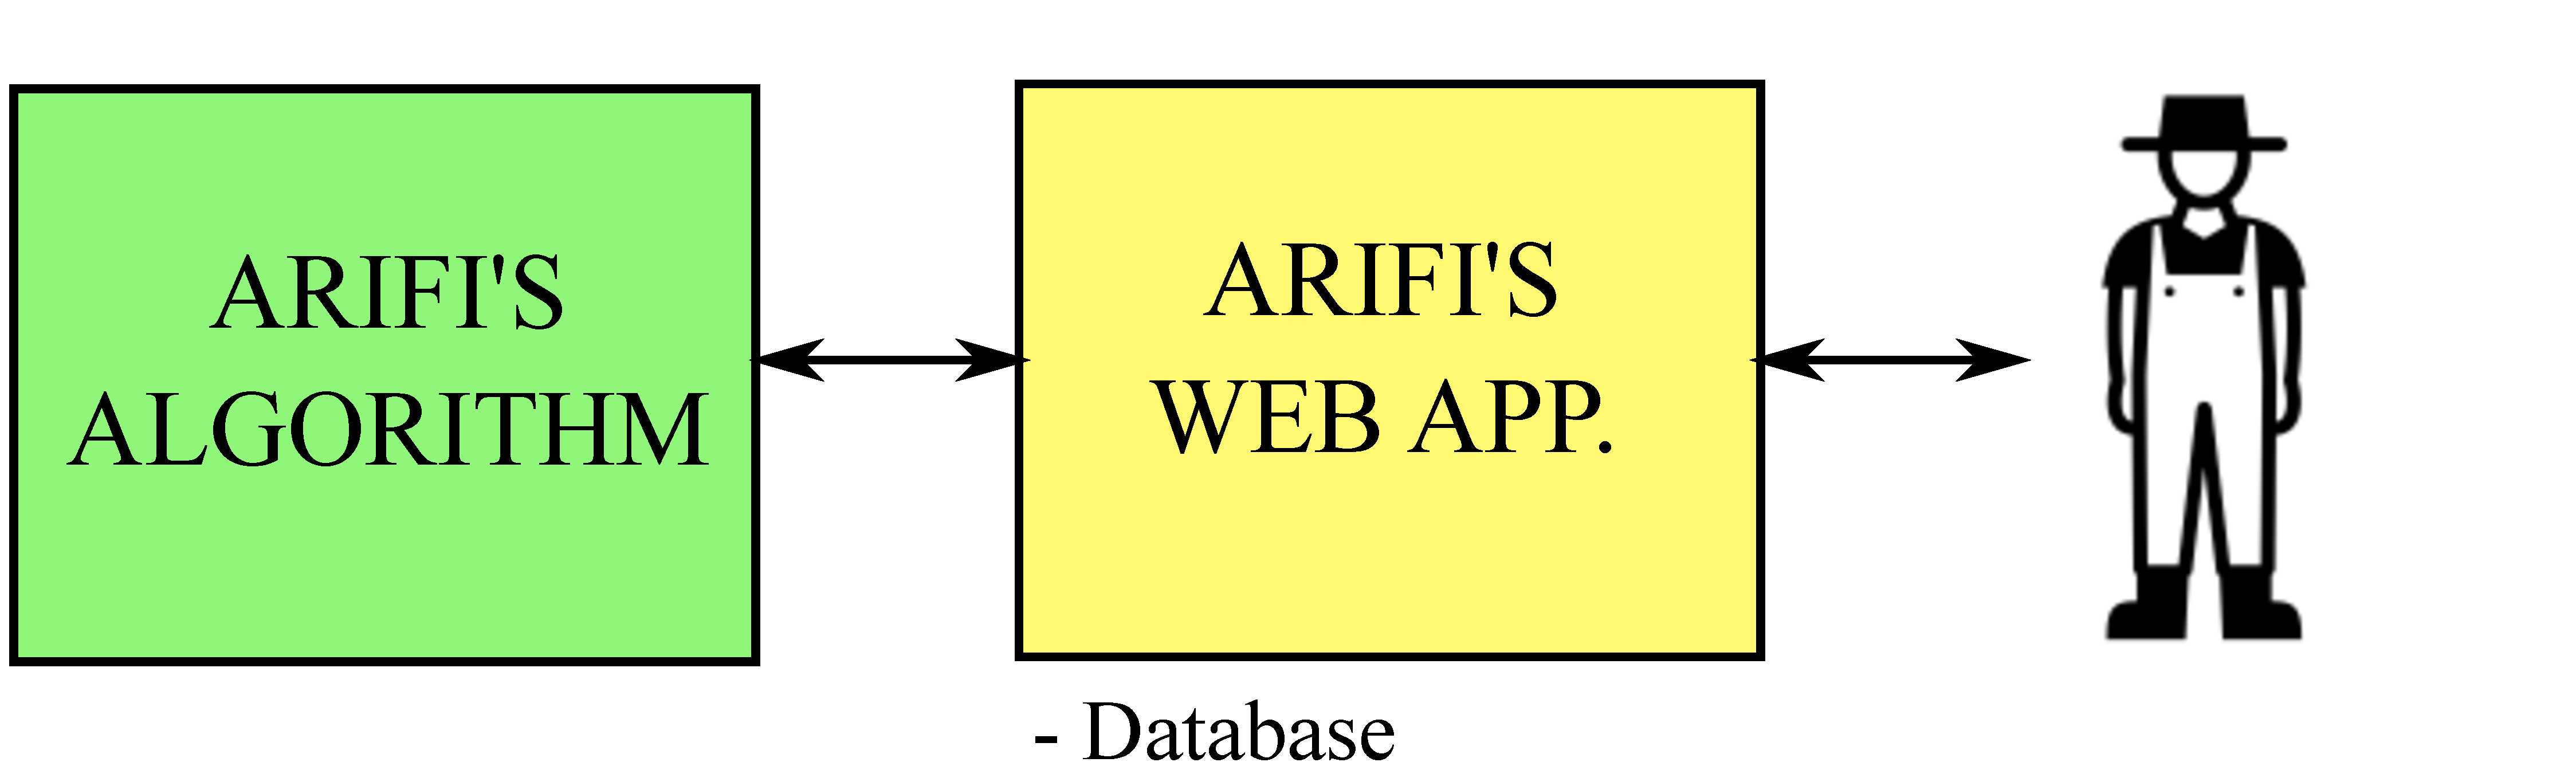
\includegraphics[scale= 0.15]{images/dibujo2.eps}
    \caption{User interaction with ARIFI's services}
    \label{fig:sch2}
\end{figure}
%
ARIFI was initially thought to work as a web application. The reason to this is that one of the major concerns from ARIFI's team, was to make this service available for a wide range of users. With this in mind, a web application was thought the best platform to work with, as it only requires a device with internet connection to access to its services. Despite this, we are opened to consider other platforms such as mobile-phone applications in the future. A graphical description of user's interaction with ARIFI is depicted in figure \ref{fig:sch2}.

\newpage
\subsection{Technical aspect}
\subsubsection{GNSS side}
\begin{itemize}
    \item \textbf{GALILEO} \color{blue} is a global satellite navigation system funded, developed and maintained by Europe which provides to European citizens independence and sovereignty, minimizing the disconnection and/or interruption of other GNSS systems (such as GPS or GLONASS). Furthermore, Galileo offers new services: search and rescue (SAR), Galileo Publich Regulated Serive (PRS) for governmental authorised users and sensitive applications and more precise position for commercial purposes.   
    
    Once Galileo is fully operational it will consists of 24 active and 6 reserve satellites. Besides, different frequency bands (see figure \ref{fig:frequency_plan} \footnote{Figure obtained from \url{https://gssc.esa.int/navipedia/index.php/Galileo_Signal_Plan}}) will be used to increase and improve the precision level, availability and timing under the most hostile condition. 
    
    \begin{figure}
    	\centering
    	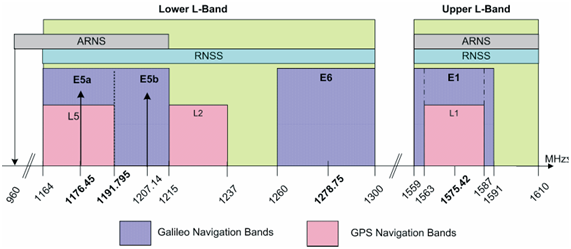
\includegraphics[width=0.8\textwidth]{images/Galileo_Frequency_Plan.png}
    	\caption{Galileo frequency distribution}
    	\label{fig:frequency_plan}
    \end{figure} 
    
    Galileo system is able to provide a position with a root-mean-square (RMS) error equals to 0.43–1.20 m, 0.52–1.29 m, and 1.34–3.25 m in the east component, north component, and up component, respectively. These errors are comparable to those obtained with GPS system despite the smaller number of satellites and larger PDOPs \cite{Gal_pos}. Obviously, these results can be improved if a precise point positioning (PPP) is used instead of the conventional standard point positioning (SPP). 

	Galileo, in combination with EGNOS (when this service is available), will be used by ARIFI in order to determinate the farmer's position within his farm and thus provide him with information on irregularities in the field. Therefore, a GNSS receiver which determinates the farmer's position is needed. Nonetheless, since ARIFI will has a wide world impact this receiver must be user-friendly and thinking in developing and least developed countries it should be cheap too. In this sense, in ARIFI project two alternatives are being evaluated
	\begin{itemize}
		\item A single chip GNSS mass market receiver as the developed under HIMALAYA project \cite{Himalaya}. However, a commercial solution could be too much expensive for the average farmer. 
		
		\item A software receiver developed and provided by the ARIFI team. So, the farmer would simply have to have a GNSS antenna and a platform to run the receiver. This option can be supplied at a cheaper price or even for free depending on the farmer's economical condition. 
	\end{itemize}
	  
	Regardless of the option chosen, the receiver will work under open sky conditions so it does not need to be a very sophisticated receiver since the only sources of error will be those given by the ionosphere and the troposphere (multipath can be considered negligible), and both effects can be easily corrected or at least mitigated. In the same way, given the open-sky condition more than 4 satellite can be easily acquired and tracked increasing the accuracy of the position. 
    
    
    \color{black} 
    \item \textbf{EGNOS}
    \item \textbf{Copernicus}
\end{itemize}
\subsubsection{AI side}
To address the proposed idea and achieve our goal, we will focus on how to relate machine learning techniques, field of Artificial Intelligence (AI), with the study of the atmosphere provided by satellite data. Thanks to the Copernicus Atmosphere Monitoring Service, we will be able to access to data that will allow us to predict the main atmospheric phenomenons which affects the production of the majority farmers.\\\\
%
In particular, we are talking about reanalysis variables. This kind of data is obtained by some weather forecasting centres, which combine past observations with a modern meteorological forecast model, in order to produce regular gridded datasets of many atmospheric and oceanic variables, with a temporal resolution of a few hours. This datasets usually extend over several decades and cover the entire planet, being a very useful tool for meteorological and climatological studies.\\\\
%
One of the most important reanalysis projects is the {\em ERA-Interim reanalysis project}, produced by the European Centre for Medium-Range Weather Forecasts (ECMWF) \cite{ERA_Interim}, which belongs to the Copernicus Programme. ERA-Interim is a global atmospheric reanalysis from 1979, continuously updated in real time.\\\\
%
Table \ref{Variables_ERA} is just an example of variables that can be obtained from this platform, which could be used as predictors in machine learning models.

\vspace{12pt}
\begin{table}[H]
\begin{center}
\caption{\label{Variables_ERA} Possible predictive variables in a prediction problem.}
\begin{tabular}{cccc}
\hline
variable name & ERA-Interim variable\\
\hline
\hline
skt & surface temperature\\
sp & surface pression\\
$u_{10}$& zonal wind component ($u$) at 10m\\
$v_{10}$& meridional wind component ($v$) at 10m\\
temp1& Temperature at 500hPa\\
up1& zonal wind component ($u$) at 500hPa\\
\hline
\end{tabular}
\end{center}
\end{table}
\vspace{12pt}

Due to the chaotic nature of atmospheric phenomenons it is so difficult predict with precision its future state. Modeling it without any un- certainty is not possible as there is a strong sensitivity to small perturbations in the initial conditions. But there is a way to overcome this issue by the use of probabilistic weather forecasts \cite{martinez2015forecasting}. In this regard, we propose computational methods belonging to machine learning techniques, a branch of AI, to get predictions or classifications over the main atmospheric factors with high accuracy. We could predict solar radiation, wind velocity, or whatever meteorological process that injures in the farmers' environment. Of course, it would not be possible without GNSS services that provide the essential dataset, as we mentioned before, necessary to train the learning models.

Many of these methods can be classified in the field of Knowledge called “Natural Computing”. The algorithms that can be found in this category are inspired by the way Nature solves complex problems. In this regard, Evolutionary Computation (EC) is inspired in the theory of evolution or Artificial Neural Networks (ANN) find their behaviour in human brain.

The conjunction between satellite data and machine learning algorithms will allow us to provide solutions to those aspects that most concern farmers, in order to keep their harvests safe with the highest possible productivity. For instance, if we are able to anticipate how much water they will have at a given time, or to warn of a dry season that was not previously contemplated but, due to the effects produced by climate change may occur, we will have a positive influence on their economy by avoiding unnecessary expenses derived from poor management, because they do not have all the information they could.

\subsection{Added value}
\subsubsection{Comparisons}	
\subsection{Discussion of critical areas}
